\section{Desarrollo de Laboratorio}
\subsection{Ejercicio N° 01: Utilizando tablas temporales de auditoría}
\begin{itemize}  \item Paso 1 conecta esta ventana de consulta a tu copia de AdventureWorksLT
				 \item Paso 2 crear una tabla temporal versionada por el sistema
				 	
					\begin{center}
    				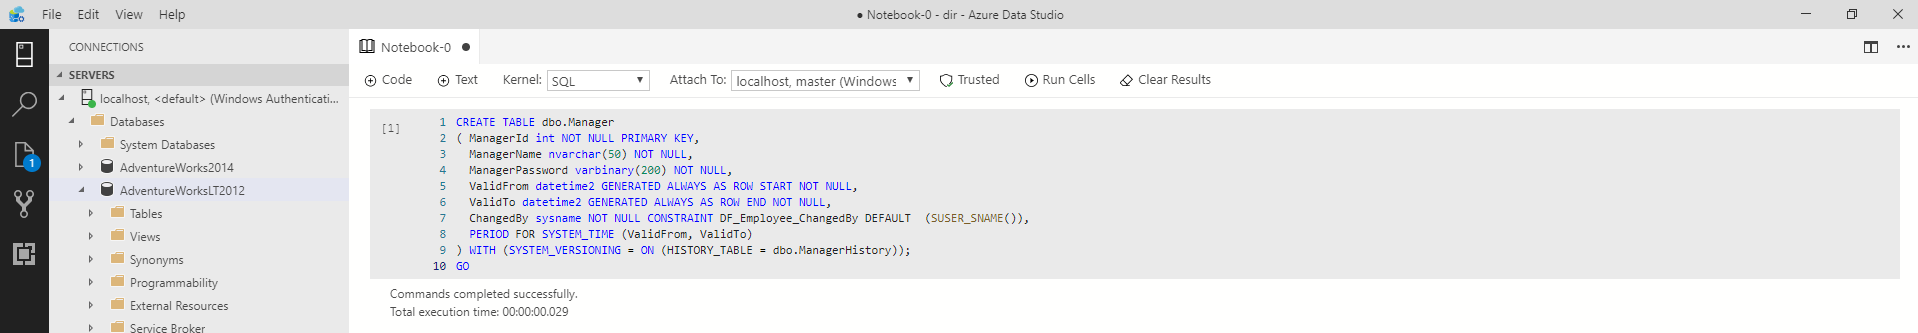
\includegraphics[width=16cm, height=90]{./Imagenes/Imagen1}
   				    \end{center}
				 

				 \item Paso 3 insertar datos de ejemplo
				 
				 	\begin{center}
    				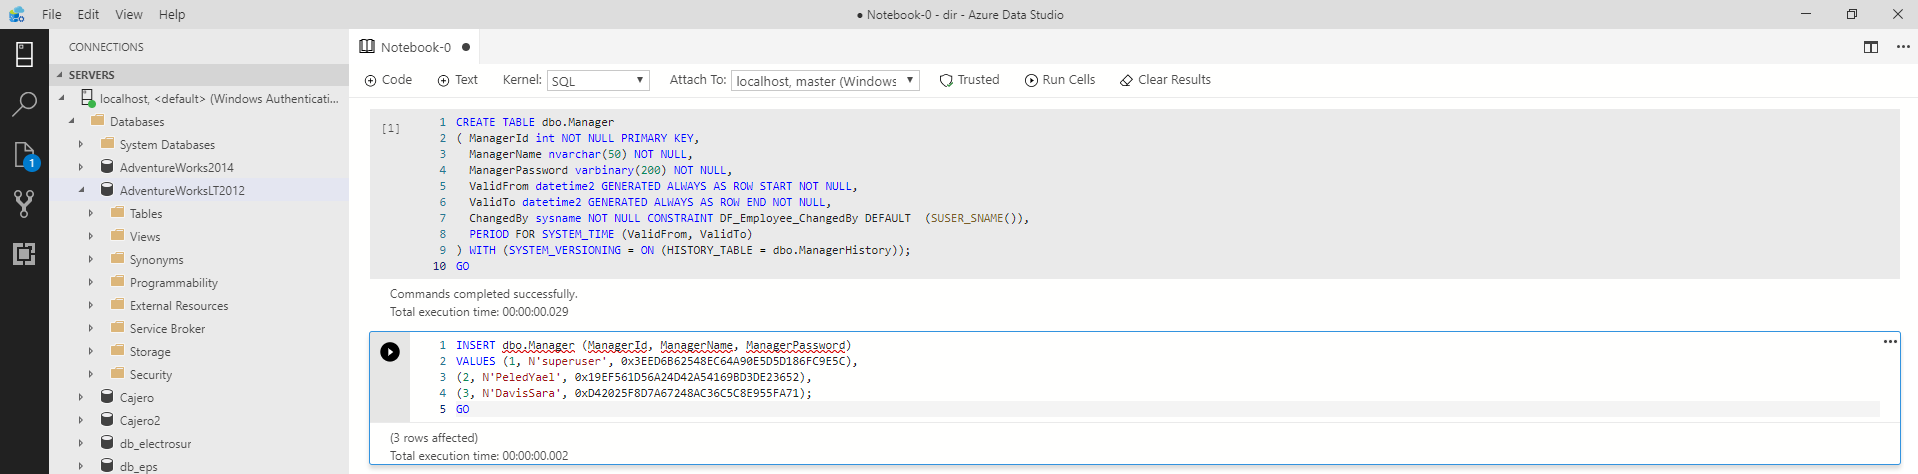
\includegraphics[width=16cm, height=90]{./Imagenes/Imagen2}
   				    \end{center}
				 
				 \item Paso 4 actualizar una fila
				 
				 
				 \begin{center}
    				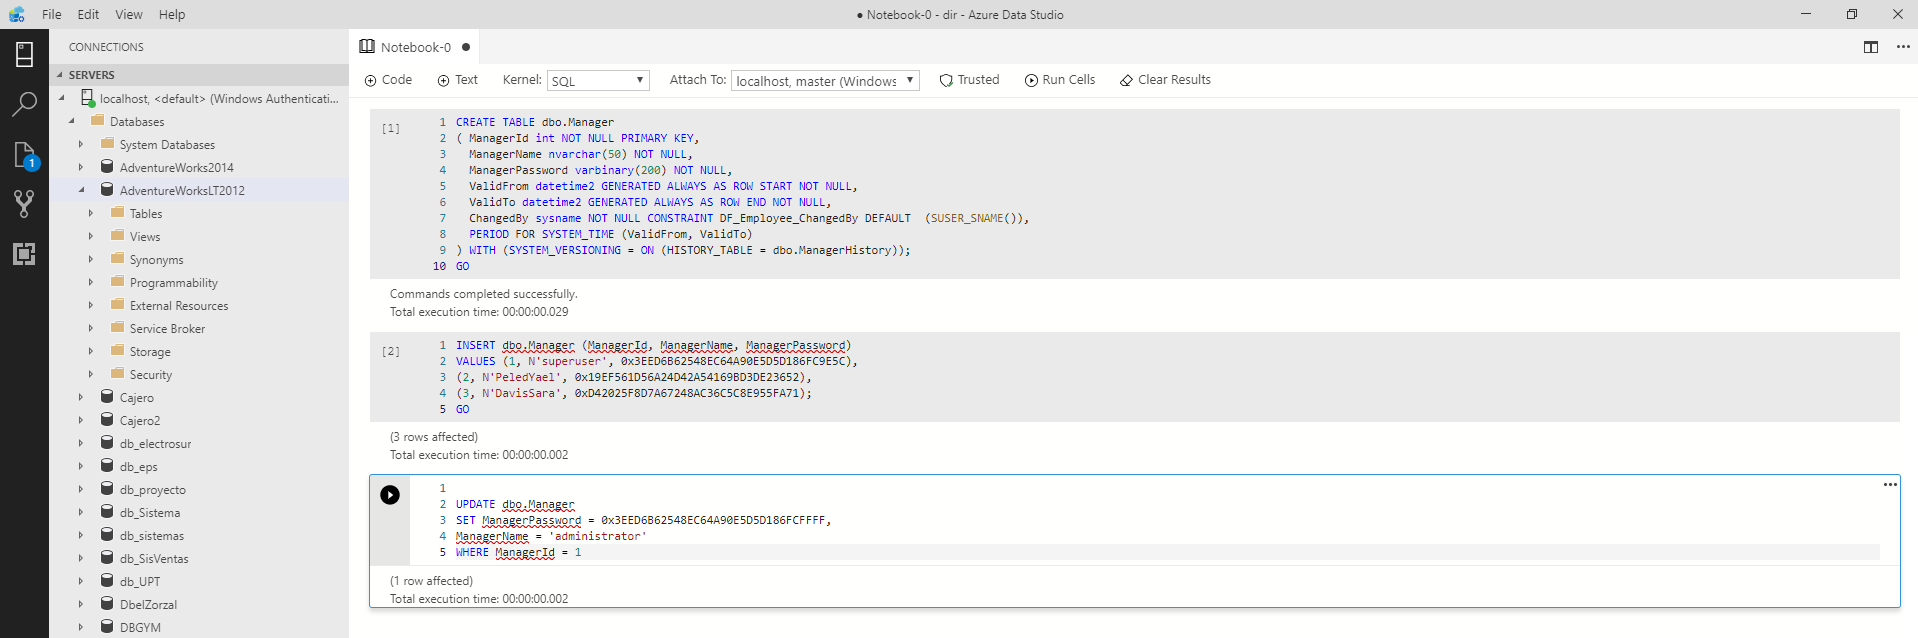
\includegraphics[width=16cm, height=90]{./Imagenes/Imagen3}
   				    \end{center}
				 
				 \item Paso 5 examinar tablas de componentes de la tabla temporal
				 
				 
				 \begin{center}
    				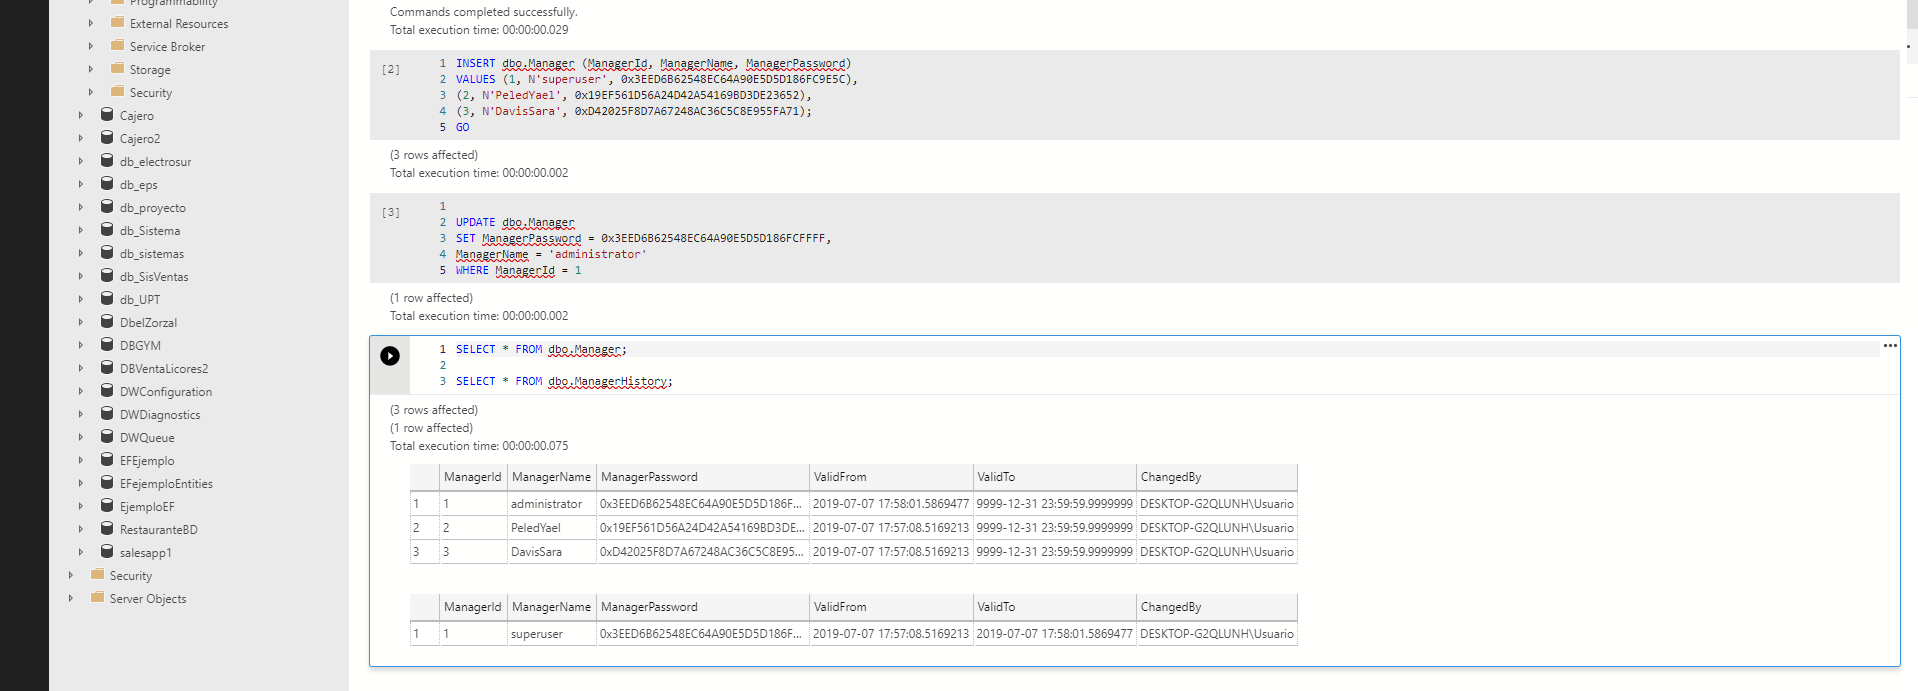
\includegraphics[width=16cm, height=90]{./Imagenes/Imagen4}
   				    \end{center}
   				    \clearpage		
   				    
   				 \item Paso 6 demuestre POR TODO EL TIEMPO DEL SISTEMA al consultar una tabla temporal TODOS muestra todos los datos en ambas tablas
				 
				 
				 \begin{center}
    				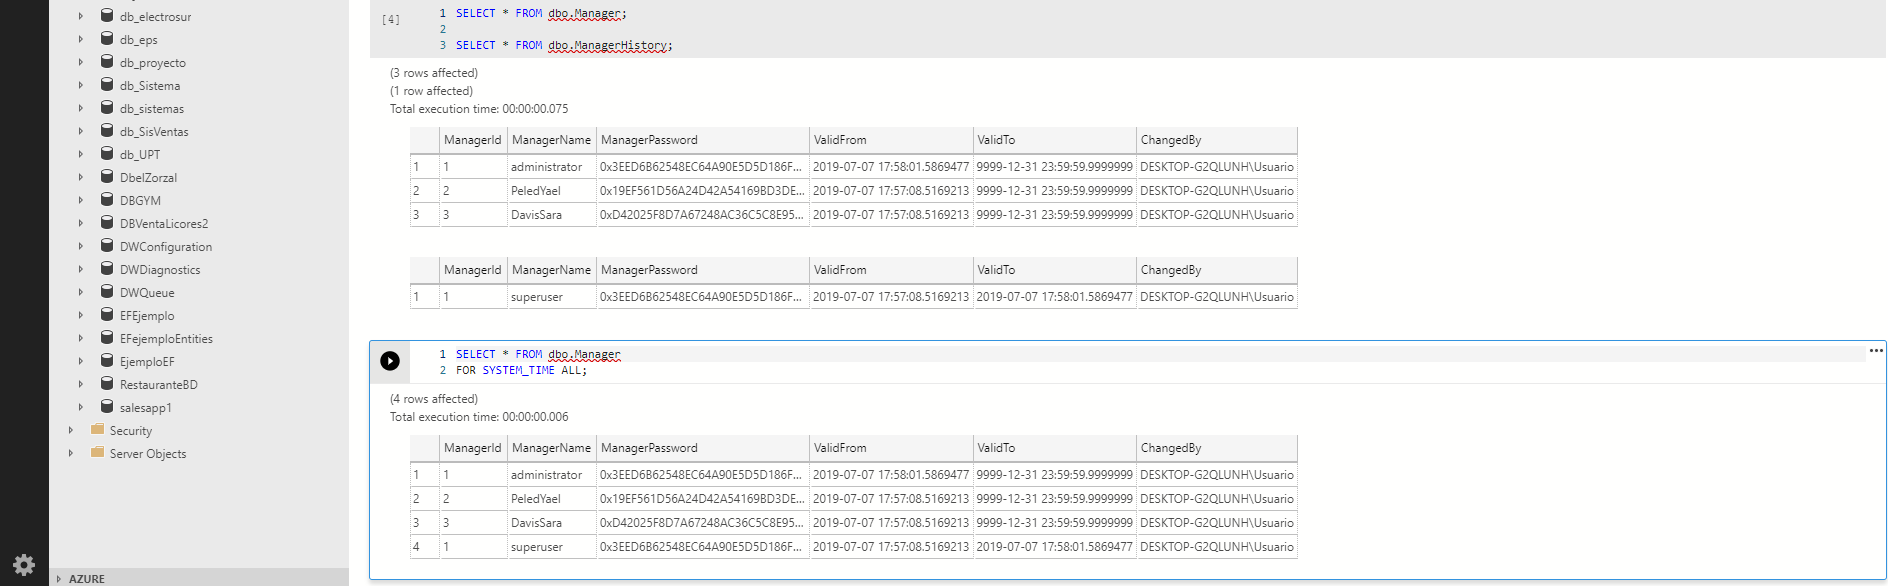
\includegraphics[width=16cm, height=90]{./Imagenes/Imagen5}
   				    \end{center}   		 
				 
				  \item Paso 7 demuestre POR TIEMPO DE SISTEMA COMO DE cuando se consulta una tabla temporal AS OF muestra un punto en el tiempo.
				 
				 \begin{center}
    				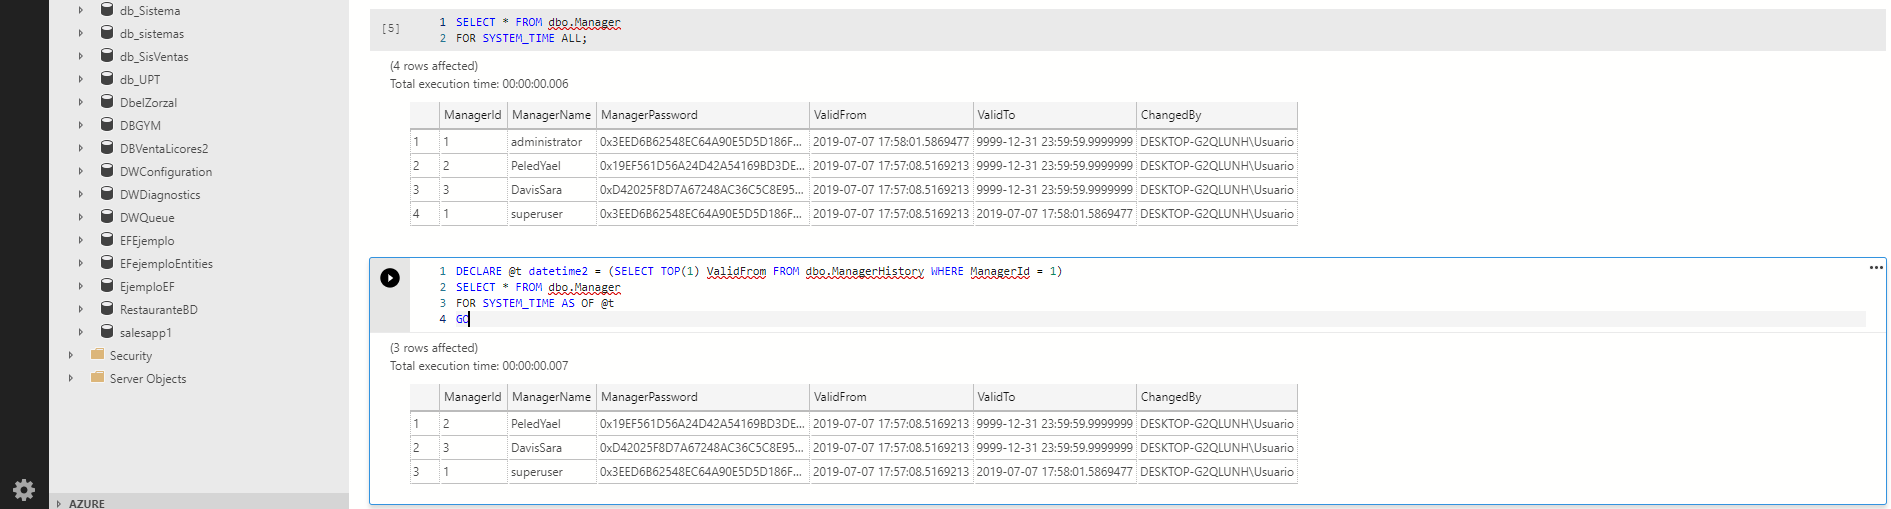
\includegraphics[width=16cm, height=90]{./Imagenes/Imagen6}
   				    \end{center} 
   				    
   				    \item Paso 8 demostrar que la tabla de historial no se puede editar (ambos comandos generarán un error)
				 
				 \begin{center}
    				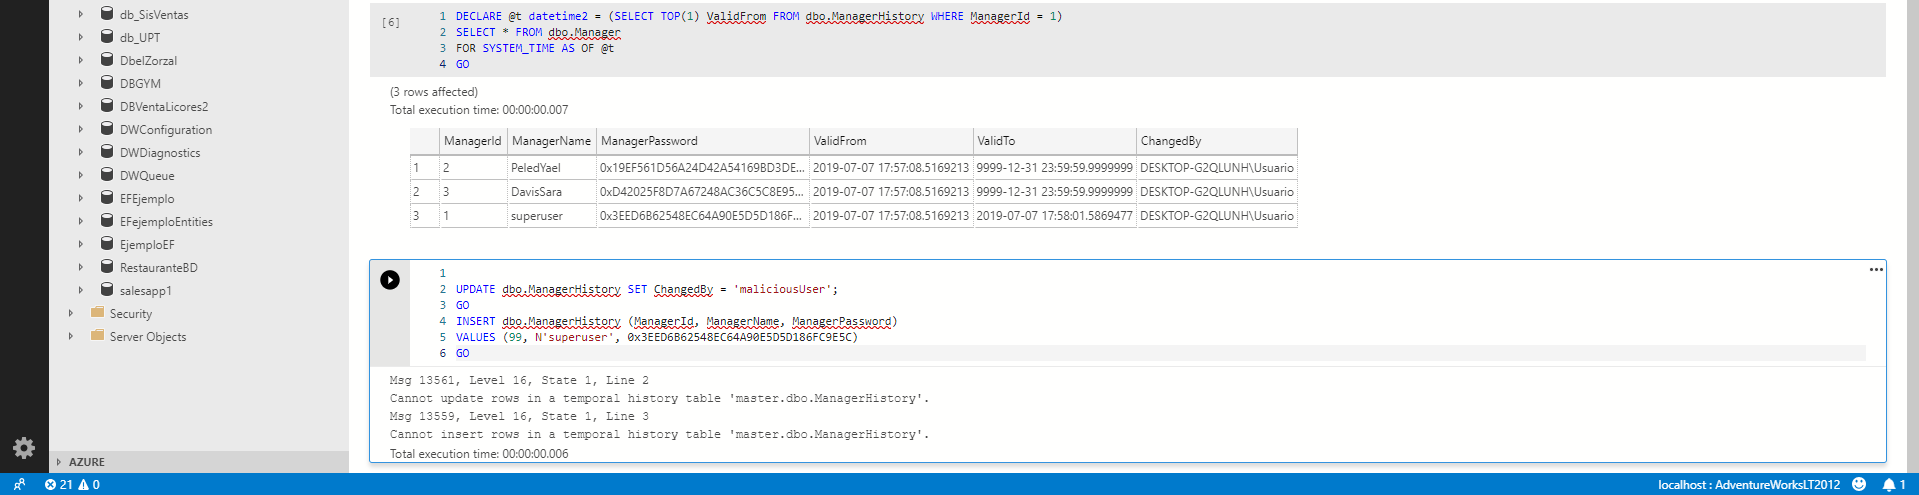
\includegraphics[width=16cm, height=90]{./Imagenes/Imagen7}
   				    \end{center}   
   				    
   				    \item Paso 9 demuestre que un usuario con permisos suficientes puede insertar datos engañosos en la columna ChangedBy:
				 
				 \begin{center}
    				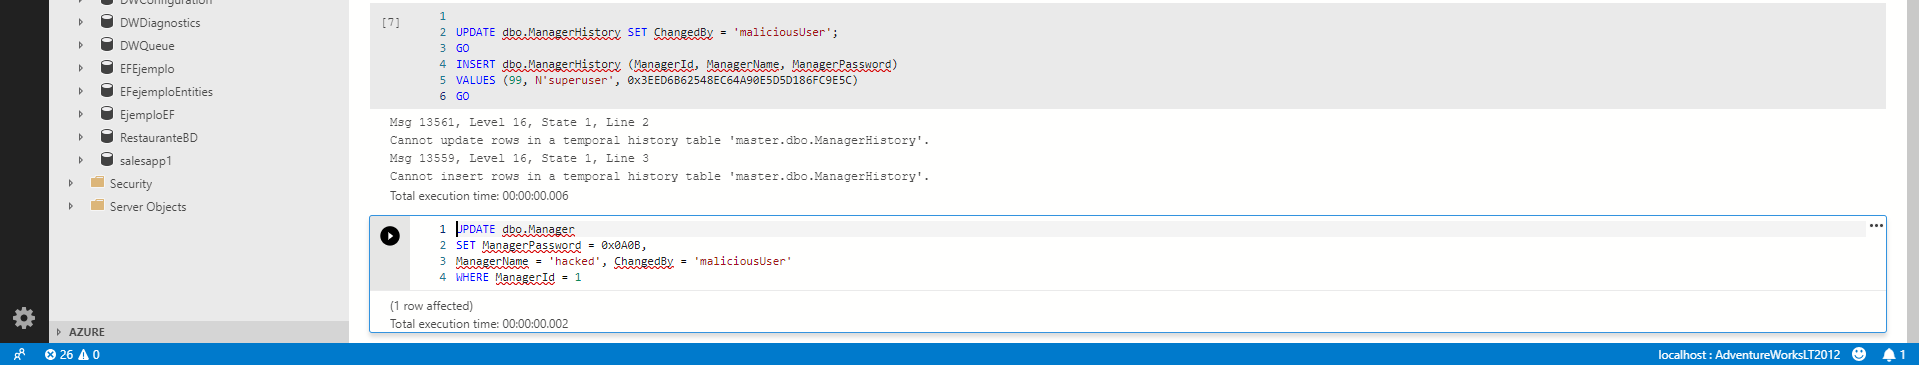
\includegraphics[width=16cm, height=90]{./Imagenes/Imagen8}
   				    \end{center}   
   				    \clearpage
   				    \item Paso 10 examinar tablas de componentes de la tabla temporal
				 
				 \begin{center}
    				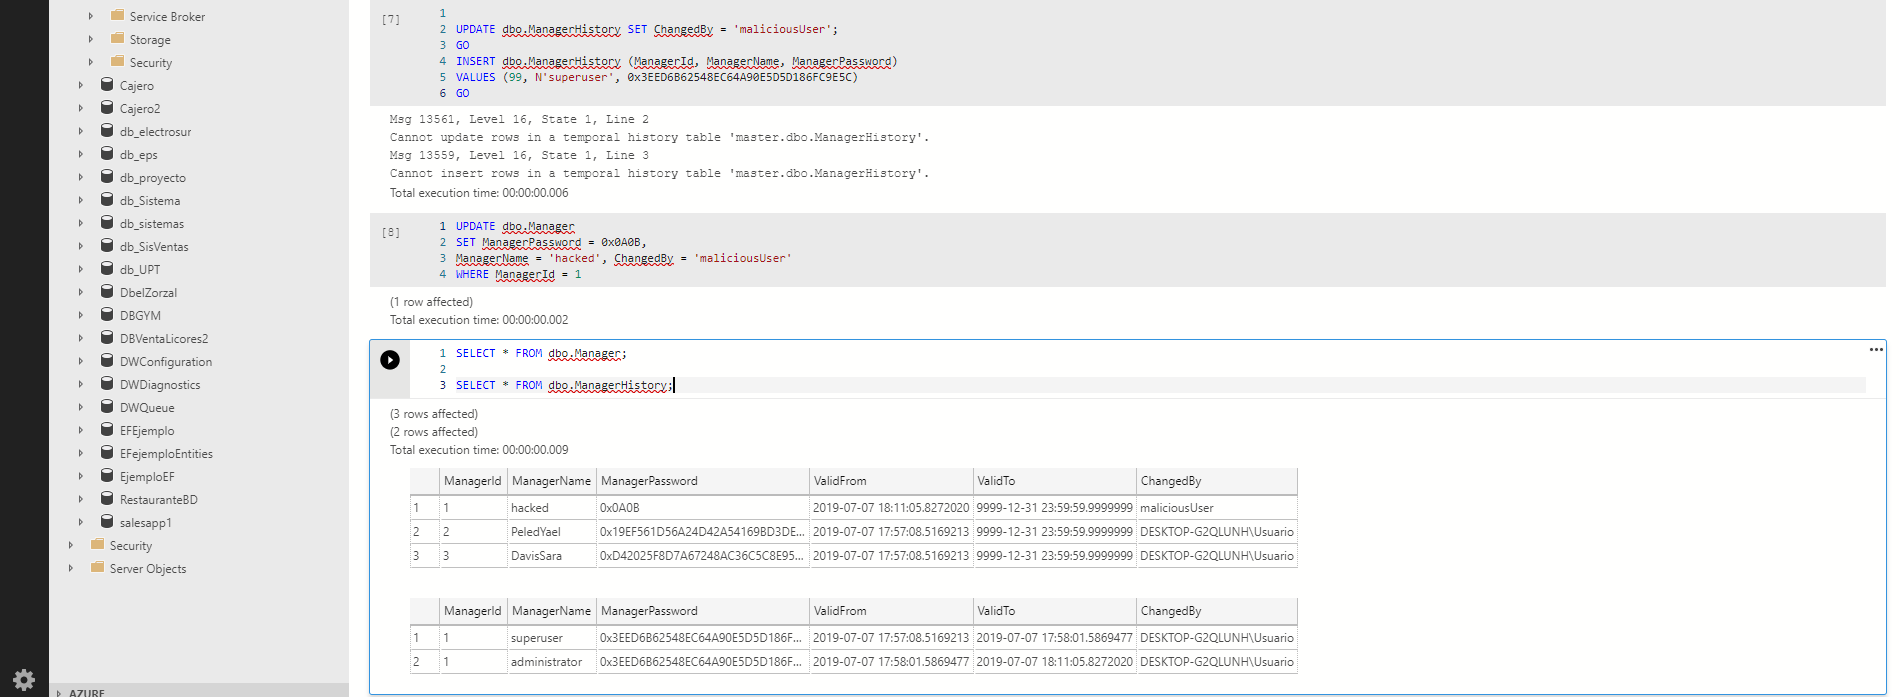
\includegraphics[width=16cm, height=90]{./Imagenes/Imagen9}
   				    \end{center} 	
   				    
   				     \item Paso 11 Cerrar objetos de demostración
				 
				 \begin{center}
    				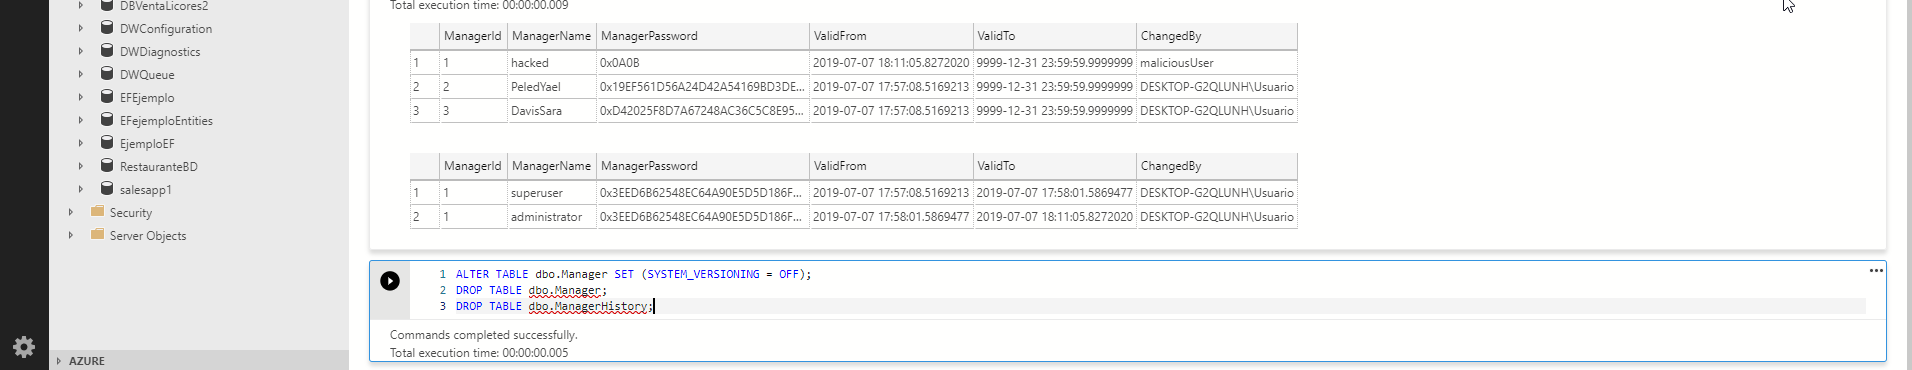
\includegraphics[width=16cm, height=90]{./Imagenes/Imagen10}
   				    \end{center} 		 
				 
				 
				 
				  
				 				  
				   \end{itemize}

\subsection{Tipos de Modelos}

\\\\




